\documentclass[tikz]{standalone}

% \usepackage{newtxtext,newtxmath}

%!TEX root = main.tex

% mytikzset
\usepackage{tikz}
\usetikzlibrary{positioning,arrows,shapes,patterns}
\usetikzlibrary{decorations.pathmorphing}
\usetikzlibrary{decorations.markings}
\usetikzlibrary{decorations.pathreplacing}
\usetikzlibrary{calc}
\usetikzlibrary{patterns}
\usetikzlibrary{decorations.markings}
\usetikzlibrary{petri}

\tikzset{
  vector/.style={thick,double,draw=black, postaction={decorate},
    decoration={markings,mark=at position .6 with {\arrow[black,scale=0.4]{triangle 45}}}},
  axial/.style={thick,double,densely dashed,draw=black, postaction={decorate},
    decoration={markings,mark=at position .6 with {\arrow[black,scale=0.4]{triangle 45}}}},
  gluon/.style={decorate, draw=black,
    decoration={coil,aspect=0.3,segment length=5pt,amplitude=3pt}},
  pseudo/.style={thick, dashed, draw=black, postaction={decorate},
    decoration={markings,mark=at position .6 with {\arrow[red,scale=0.5]{triangle 45}}}},
  scalar/.style={thick,draw=black, postaction={decorate},
    decoration={markings,mark=at position .6 with {\arrow[black,scale=0.5]{triangle 45}}}},
  cut/.style={draw=black, decorate, decoration={snake, segment length=1mm, amplitude=0.2mm}}
}

\definecolor{myGreen}{RGB}{0,127,0}

\begin{document}
\nopagecolor
  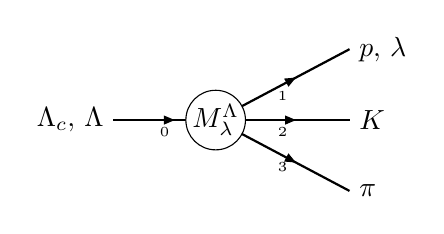
\begin{tikzpicture}[node distance=0.9cm and 1.3cm, baseline=1cm]
    \coordinate[] (c0);
    \coordinate[left=of c0,label= left:{$\Lambda_c,\,\Lambda$}] (Lamc);
    \coordinate[above right=of c0, xshift=4mm, label=right:{$p,\,\lambda$}] (p);
    \coordinate[below right=of c0, xshift=4mm, label=right:{$\pi$}] (pi);
    \coordinate[      right=of c0, xshift=4mm, label=right:{$K$}] (K);

    \draw[scalar]  (Lamc) -- node[yshift=-1.5mm] {\tiny $0$}  (c0);
    \draw[scalar]  (c0) -- node[yshift=-1.5mm] {\tiny $1$} (p);
    \draw[scalar]  (c0) -- node[yshift=-1.5mm] {\tiny $2$} (K);
    \draw[scalar]  (c0) -- node[yshift=-1.5mm] {\tiny $3$} (pi);

    \draw[black, fill=white] (c0) circle (2.5ex) node[] {$M^{\Lambda}_{\lambda}$};
  \end{tikzpicture}
\end{document}
